\chapter{Cell assemblies analysis}
\label{chap:AssemblyAnalysis}
\begin{figure}
    \centering
    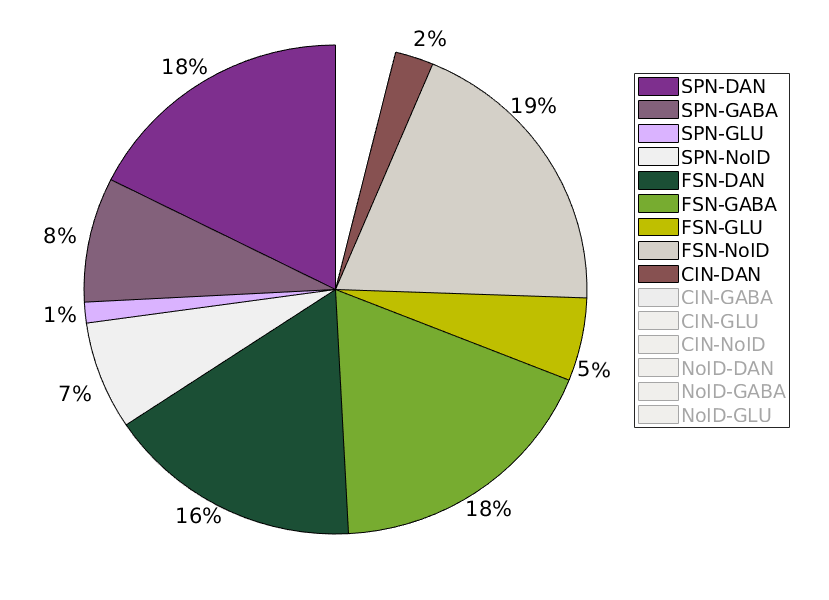
\includegraphics[scale=0.6]{figures/PieAssemblies1.png}
    \caption{Pie charts of assemblies types. We have four principal inter-regional assemblies types. }
    \label{fig:PieAssemblies}
\end{figure}
Preliminary cell assemblies analysis were aimed to understand the size of the concentration of the shared pairs, namely how many units are involved in pairs and, among those, how the units typologies were distributed in assembly pairs. Classified units were distributed in the two regions as shown in fig. (\ref{fig:PieAssemblies}) {\color{red} to be rephrased}. Performing a Pearson's Chi square test...{\color{red} test results}

{\color{red} Include figure pie charts for all reversal paradigma}
\section{Time scales, directionality}
Applying the cell-assembly algorithm we were able to detect synchronous ($lag=0$) and asynchronous ($lag\neq 0$) cell assemblies at arbitrary time scale ($\Delta$). Time scales distribution results to be different for intra- regional assembly pairs (pairs with units from VS or VTA) and inter-regional assemblies pairs (pairs with units from both VS and VTA). It's important to point out that, in case of inter-regional pairs, the lag distribution it's a instruments to measure directionality between two regions, indicating which unit fires first, leading the activation pattern activity, and which one consequently follows. In our case $lag >0$ means VS precedes in activity VTA, and $lag <0$ the opposite, $lag=0$ means that the two units are  simultaneous in activation at the precision of the time scale at which they were detected.
We start our analysis from time scales distribution involved in detection pairs.
\begin{figure}[H]
\centering
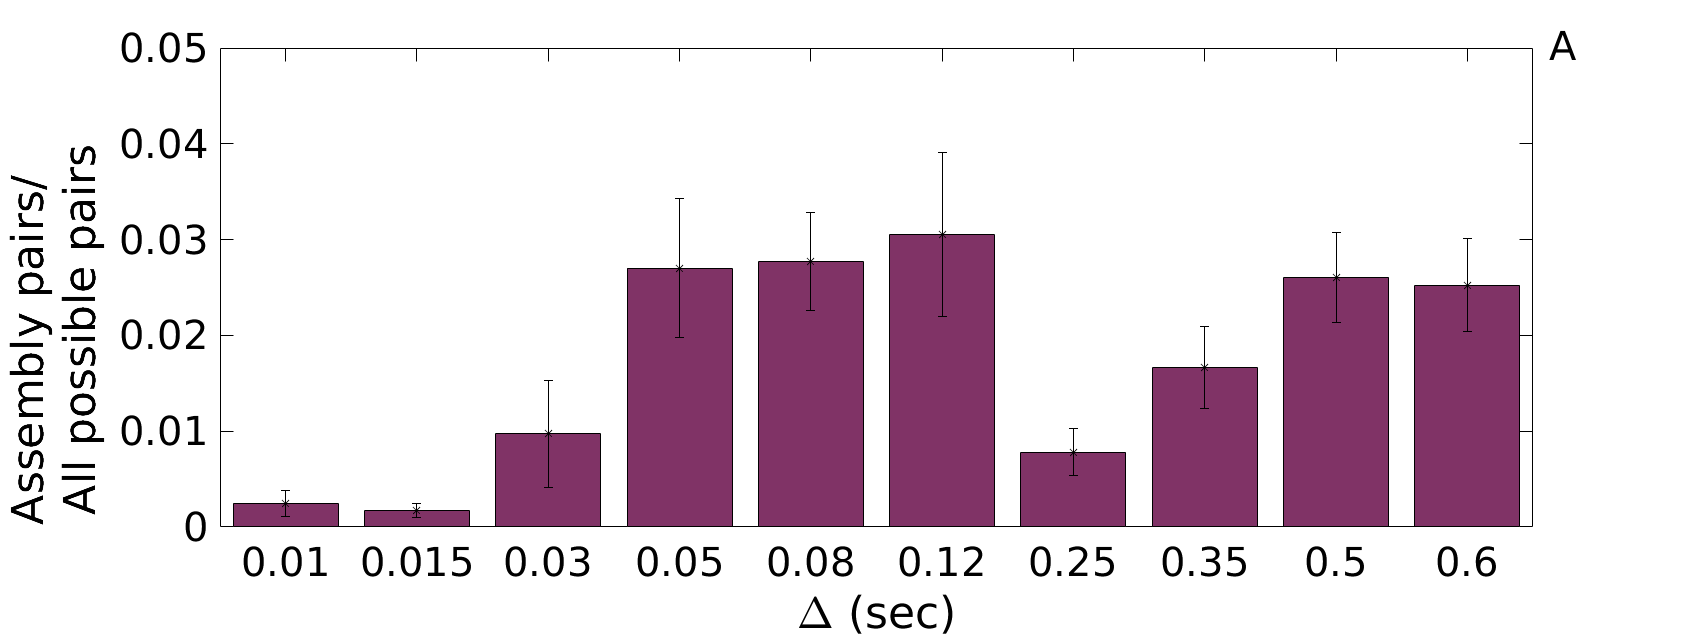
\includegraphics[scale=0.2]{figures/VS_VTA_SLet.png}
%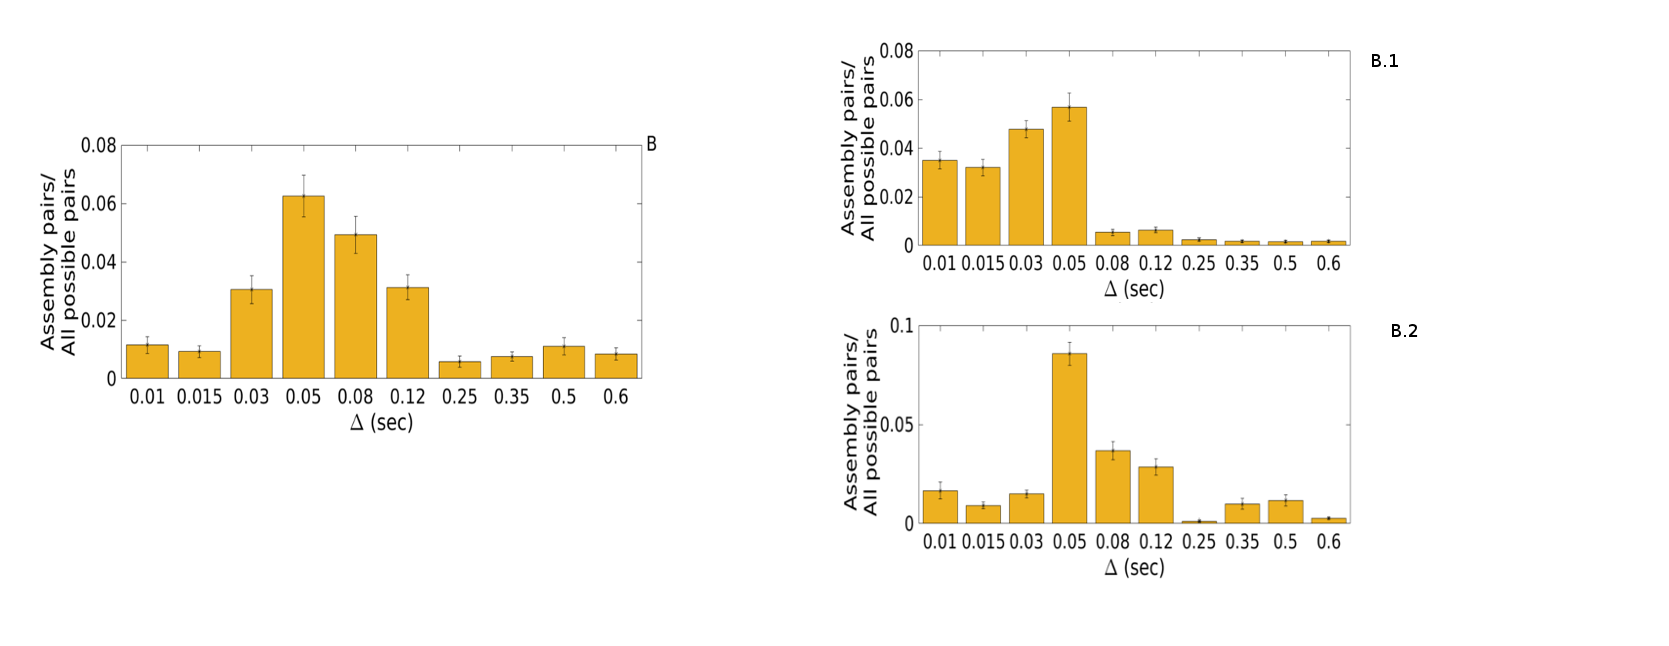
\includegraphics[scale=0.4]{figures/VS_VS_SLet1.png}
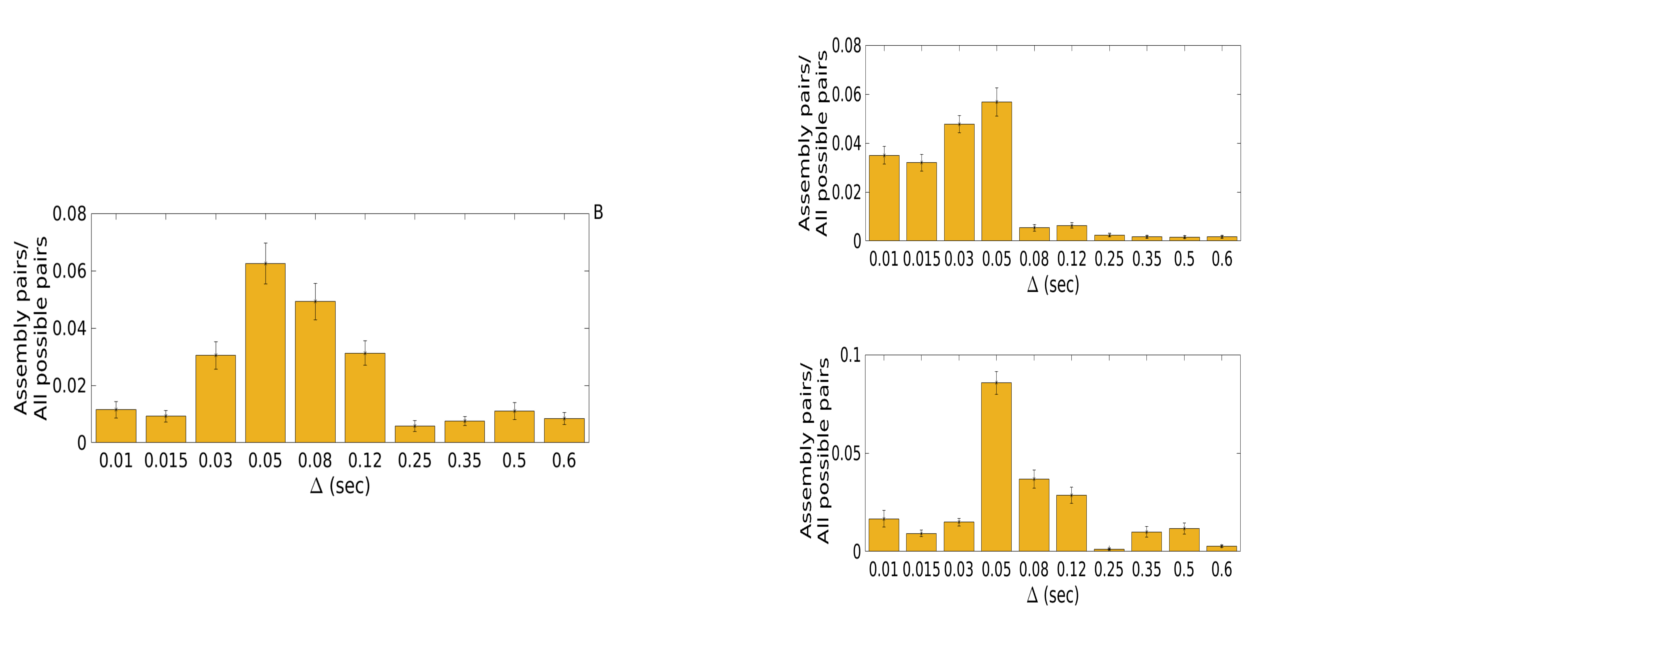
\includegraphics[scale=0.4]{figures/AllBinVSVS.png}
%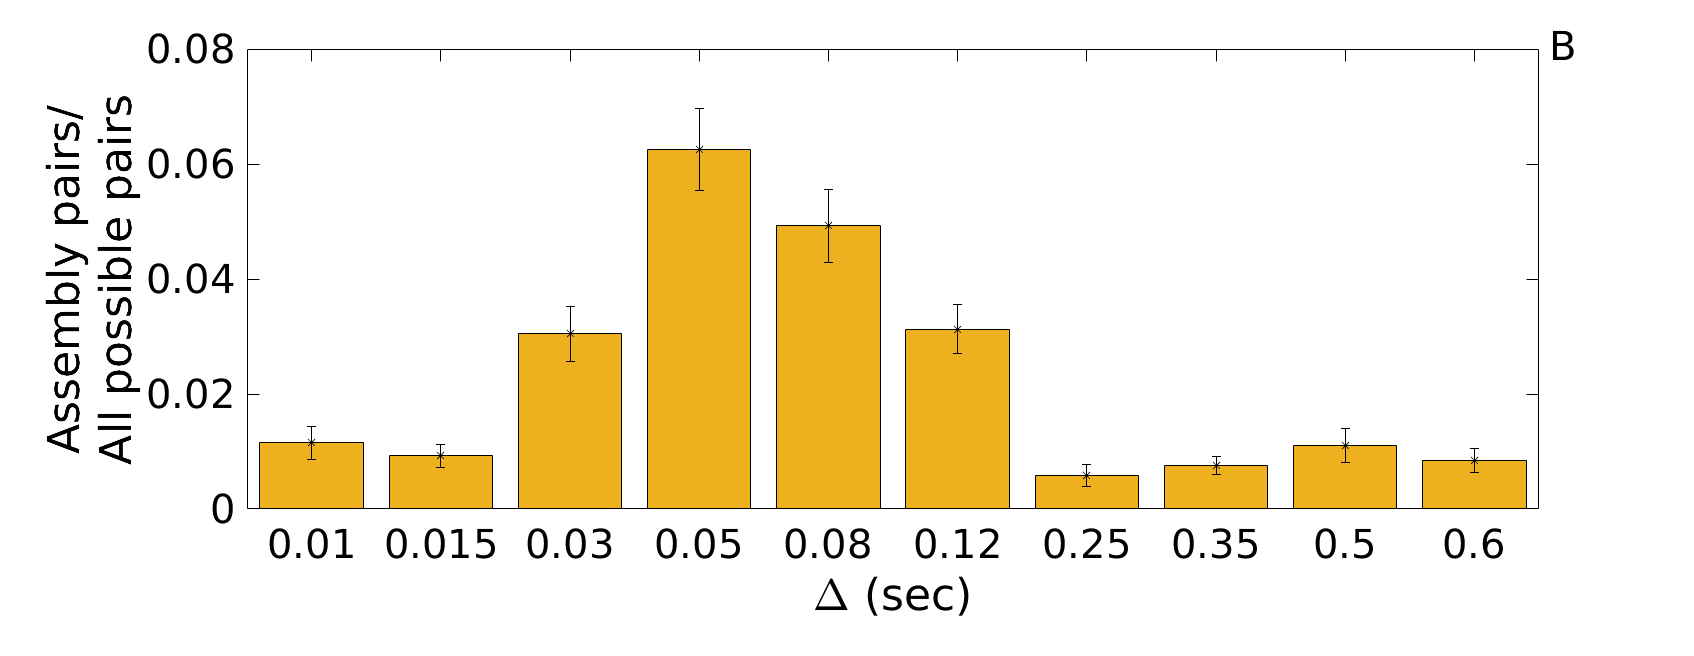
\includegraphics[scale=0.2]{figures/VS_VS_SLet.png}
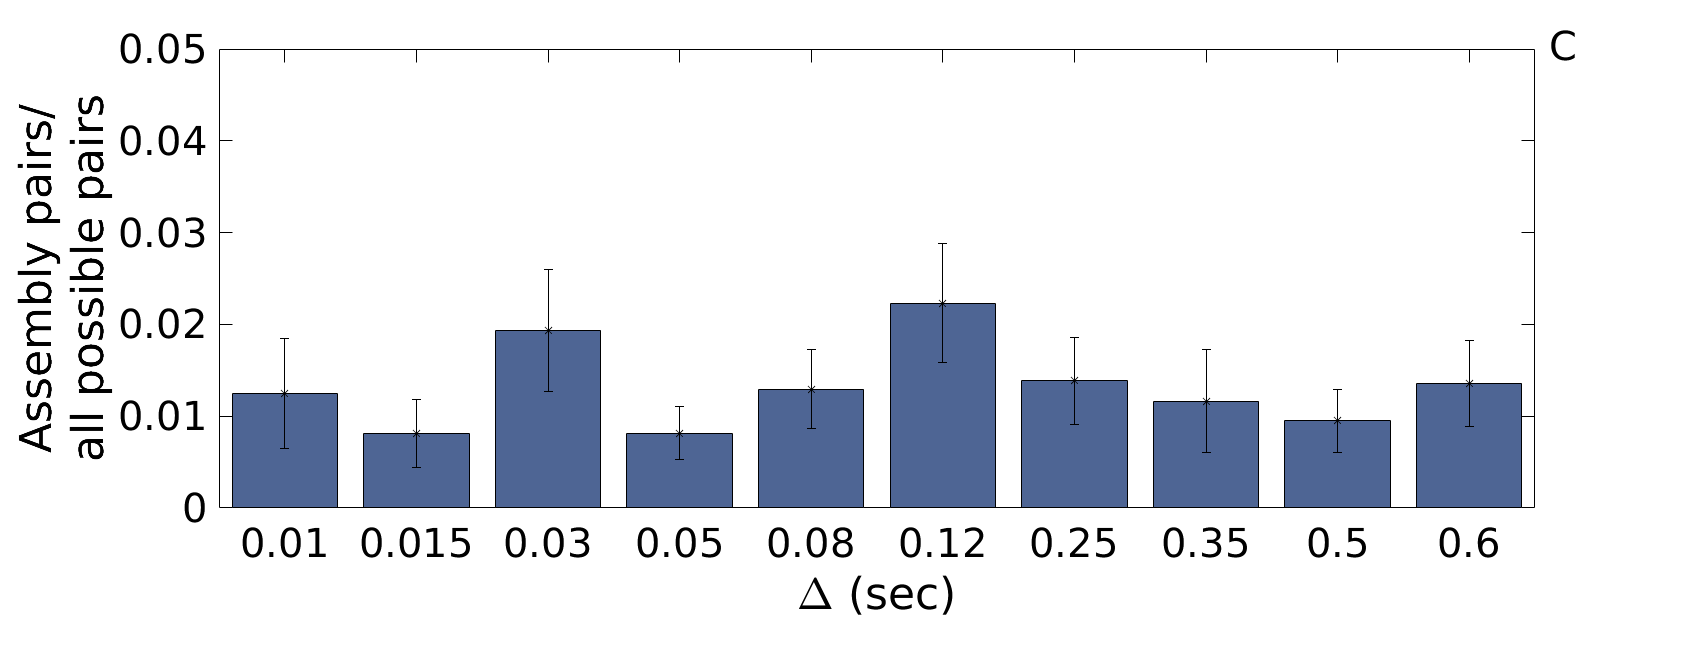
\includegraphics[scale=0.2]{figures/VTA_VTA_SLet.png}

\caption{{\color{red}Important!! Re do the figures with GIMPS include text with title} Bin distribution for intra-regional and inter-regional pairs. A) VS-VTA pairs show a bimodal distribution, meaning two temporal scale involved in inter-regional activtion patterns. B) VS-VS pairs bin distribution presents a peak at 50 $ms$, specifically in this region the pairs MSN-FSI high show an highly peaked distribution, almost centered at the peak of 50 $ms$, plot (B.2), while in MSN-FSI low distribution, albeit the peak is still at 50 $ms$, is evident the predominance of very precise time scales, including bins from 10 $ms$ to 50 $ms$, with respect to the larger time scale plot (B.1).}
\label{fig:BinDistr}
\end{figure}
Clear differences in time scales distribution of pairs detected in VS, VTA and VS-VTA emerge in fig.(\ref{fig:BinDistr}). While we observed assemblies of temporal precision at the scale of few tens of milliseconds only within either VS or VTA, assemblies of lower temporal precision were detected across VS-VTA units. The temporal precision of this last group displayed a bimodal distribution with peaks around $80$ milliseconds and one $1.6$ second, revealing the presence of two time scales, the first, preciser, ranged from 10 $ms$ to 250 $ms$, and the second including broader bin sizes. Intra-regional VTA-VTA pairs instead don't present any peak in time scales distribution. Intra-regional VS-VS bin size distribution is peaked around 50 $ms$. In VS we noticed differences between MSN and high-firing-rate FSI pairs and MSN and low-firing-rate FSI bin size distributions: specifically the firsts show higher temporal precision than the latter. {\color{red}{Include Figure of MSN-FSI and caption of bin size distribution}}.
Bin width and lags analysis reveals time scale segregation, that can reveal in turn different assembly-activation patterns. In fig.(\ref{fig:AsActBinLag}) heat maps of assembly activity, detected in a particular paradigm, show differences in activation patterns among different bin width and lag. %% In the paradigm in examination animals were well-trained, it was the third time that the same couple of odor were presented with the same stimulus duration length.
\begin{figure}
    \centering
    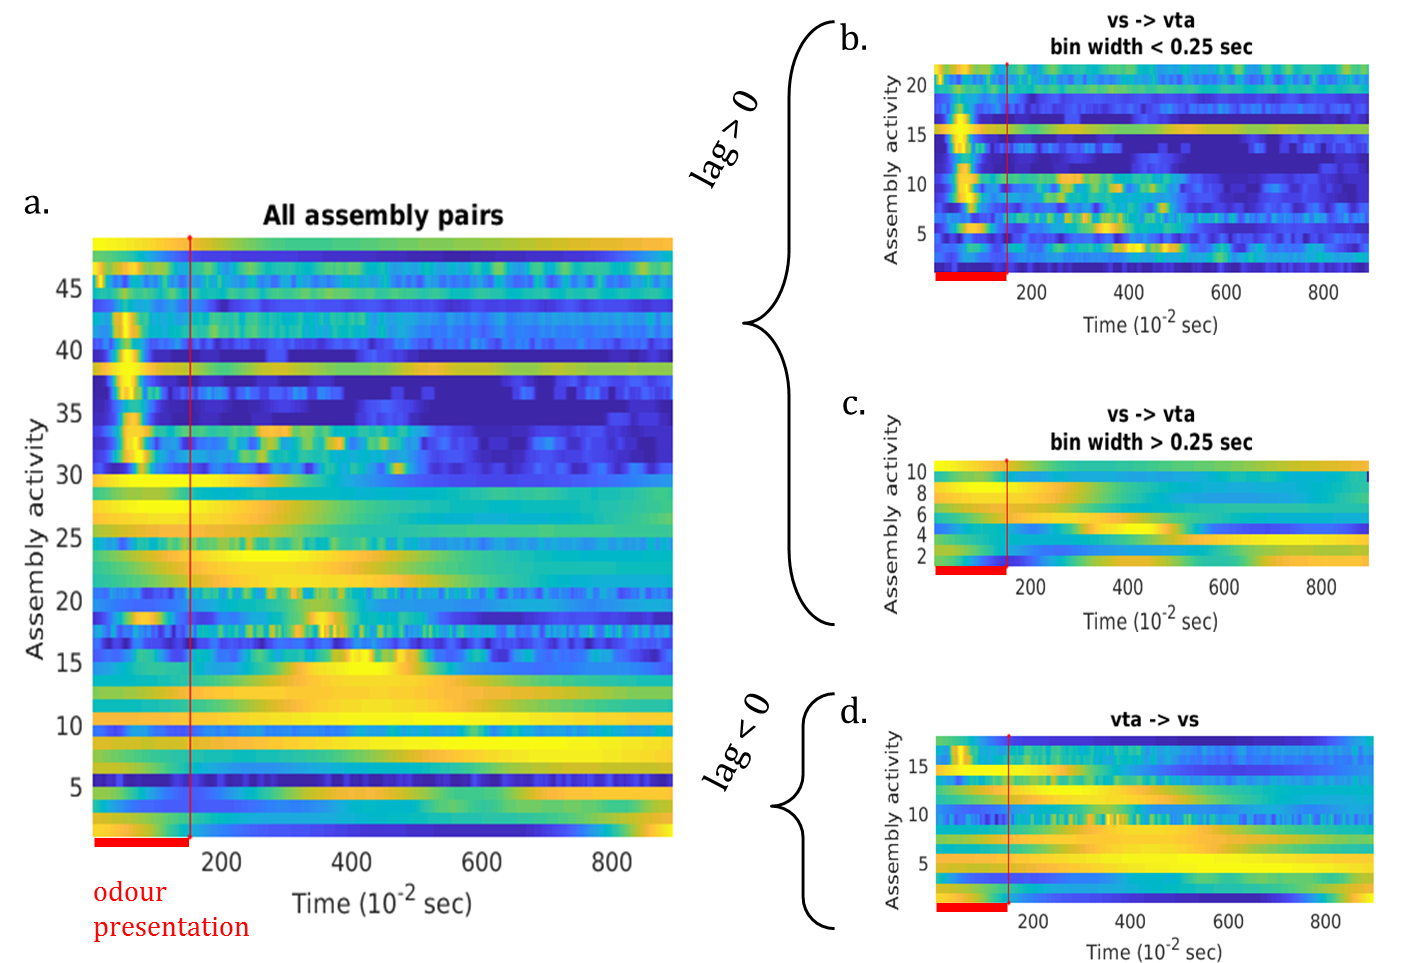
\includegraphics[scale=0.45]{figures/AsActPerBinLag1.png}
    \caption{Assembly-activation patterns given time bins and lags. In a.) totality of assemblies of one experimental paradigm, b,c,d. assemblies of same paradigm of a. selected for bin size ($\Delta$) and lag, $\Delta < 0.25 s$ and $lag > 0$ (b.), $\Delta > 0.25 s$ and $lag > 0$ (c.), $lag < 0$ (d.)}
    \label{fig:AsActBinLag}
\end{figure}
{\color{red}Include fig with all reversal paradigm and see which differences can be mentioned!!!}
The considerations above on the time scales distribution led us to study separately lag distribution of VS-VTA pairs detected in preciser and broader temporal scales highlighted from bin sizes distribution. We divided then these two assemblies population for the further study of directionality.
Interestingly lag distribution of precise and broad time scales are both asymmetric, indicating that the VS activation leads the activation of the VTA neuron (fig. \ref{fig:LagInSecAll}). The two distribution show however remarkable differences: broader time scales pairs show a fat-long tailed distribution, whereas precise time scales lag distribution.
Focusing our study on the more precise inter-regional pairs, we observed that specifically, the directional assemblies were composed of striatal and pallidal projection neurons leading dopaminergic VTA neurons (MSN and Type I pairs). Importantly, inter unit activation lags of assemblies containing pallidal neurons (FSI) were shorter than those containing striatal projection neurons (MSN), compatibly with assumed connectivity.
\begin{figure}[H]
\centering
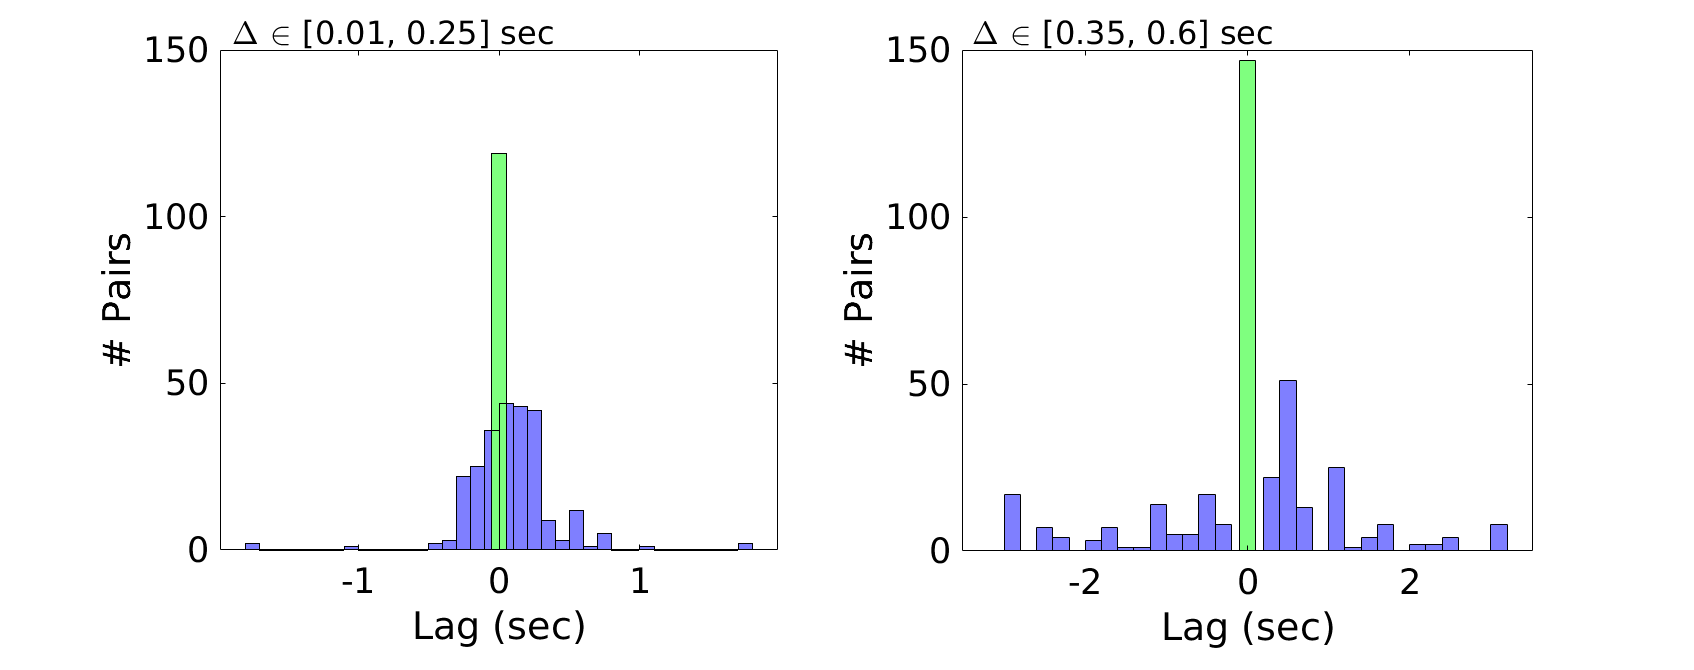
\includegraphics[scale=0.3]{figures/LagGeneralInSec.png}
\caption{Lag distribution for VS-VTA pairs in seconds. In green the synchronous pairs. On the left, lag distribution for pairs detected in preciser time scales. Slight distribution asymmetry indicates directionality in the direction of $lag > 0$, meaning a predominance of pairs in which VS leads VTA. On the right, the lag distribution for pairs detected in the broader time scale.}
\label{fig:LagInSecAll}
\end{figure}

\begin{figure}[H]
\centering
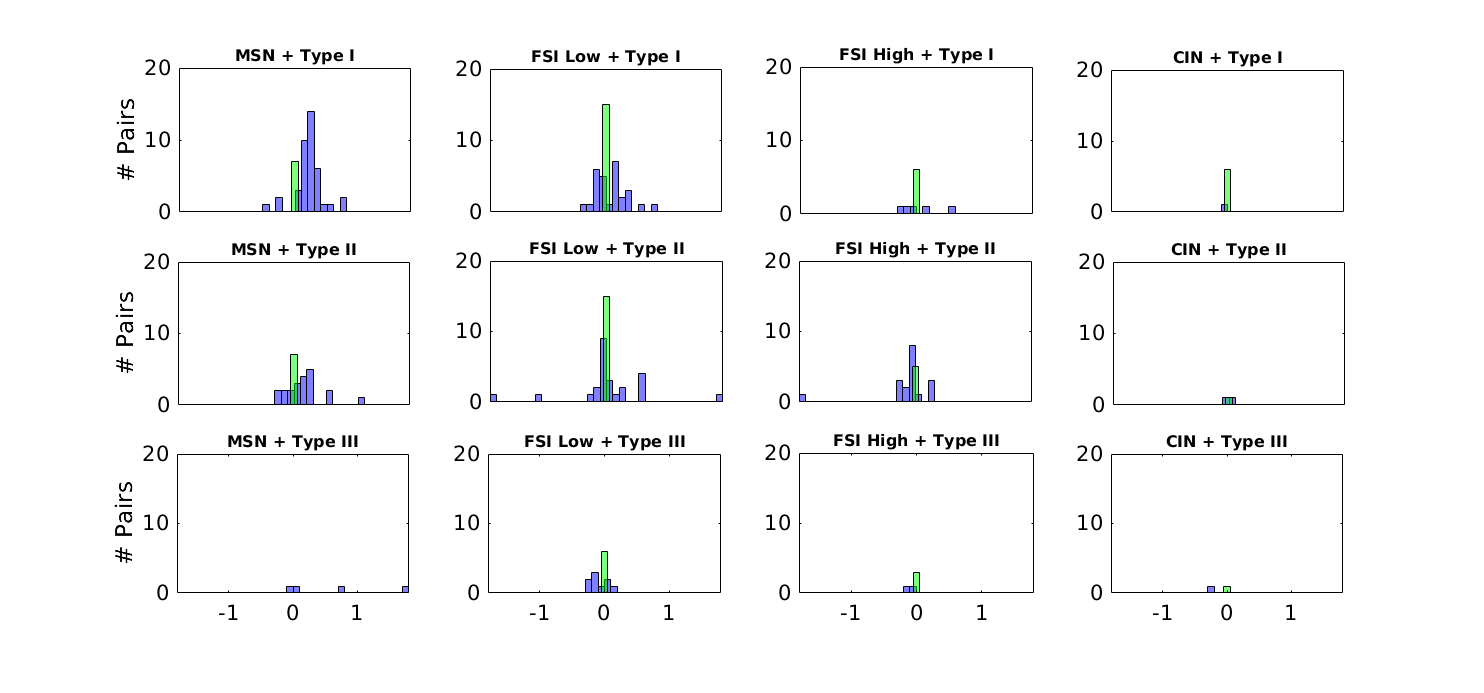
\includegraphics[scale=0.4]{figures/Type_oriz.png}
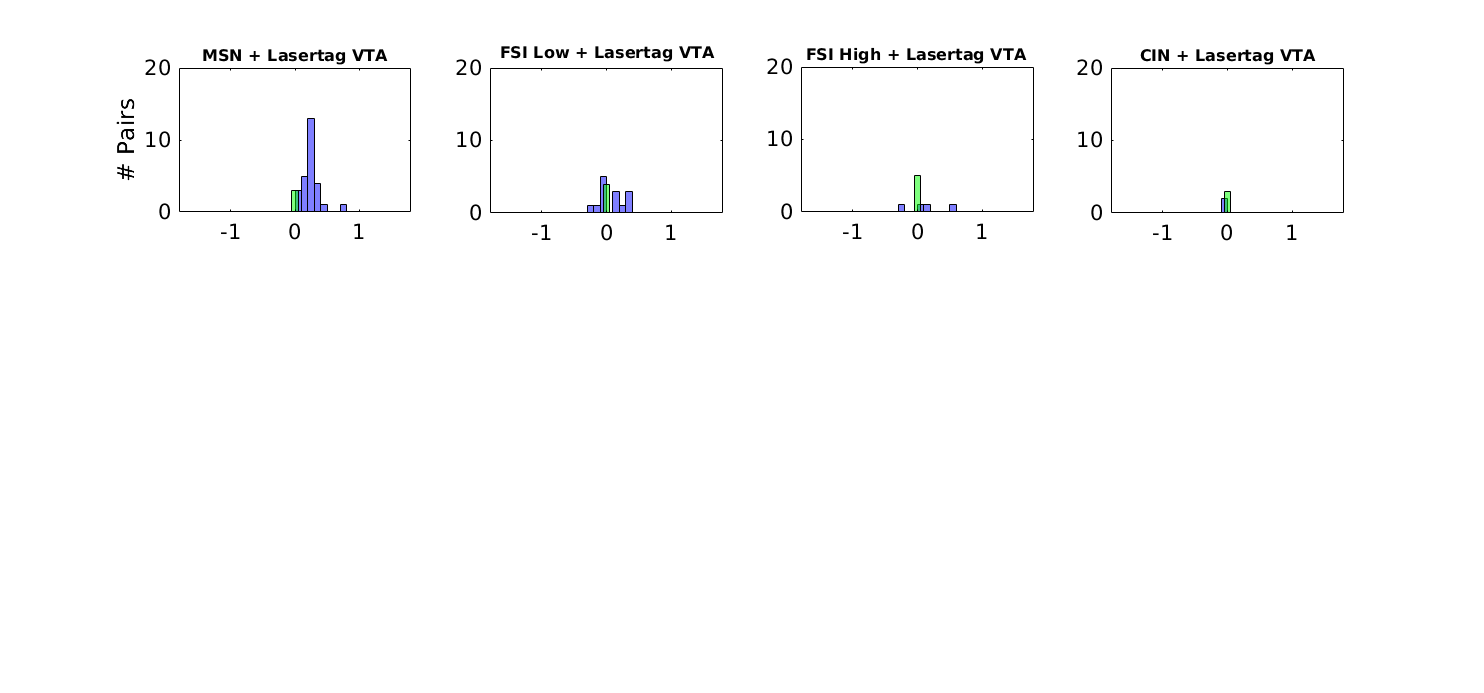
\includegraphics[scale=0.4]{figures/OnlyLaserOriz.png}
\caption{blabla}
\label{fig:LagInSecAll}
\end{figure}
In fig. (\ref{fig:directional_assembly}) a directional assembly. On top is shown mean and standard deviation of the assembly's activity for paired (grey line) and unpaired odor trials (purple line) in the original phase. On bottom raster plot and firing rate (mean and standard deviation) of units in assembly. x-axis origin correspond to the odor onset, while the red line marks the end of the stimulus duration. The examined assembly has a positive lag, that means VS preceding in activity VTA, from neuronal activity we can see in fact the VS unit activate before than the VTA unit. The assembly was detected with a bin size of $0.25 sec$, meaning that we are in the small temporal scale domain, in which the directionality clearly emerged. From the raster plot is evident that this kind of activation was persistent in each trial, in fact that assembly showed a significant task related activity after the stimulus. In term of assembly coding capability it is interesting to note the different activation for paired odor trials and unpaired odor trials, revealing the odor discrimination capability of the assembly. 
\begin{figure}
    \centering
    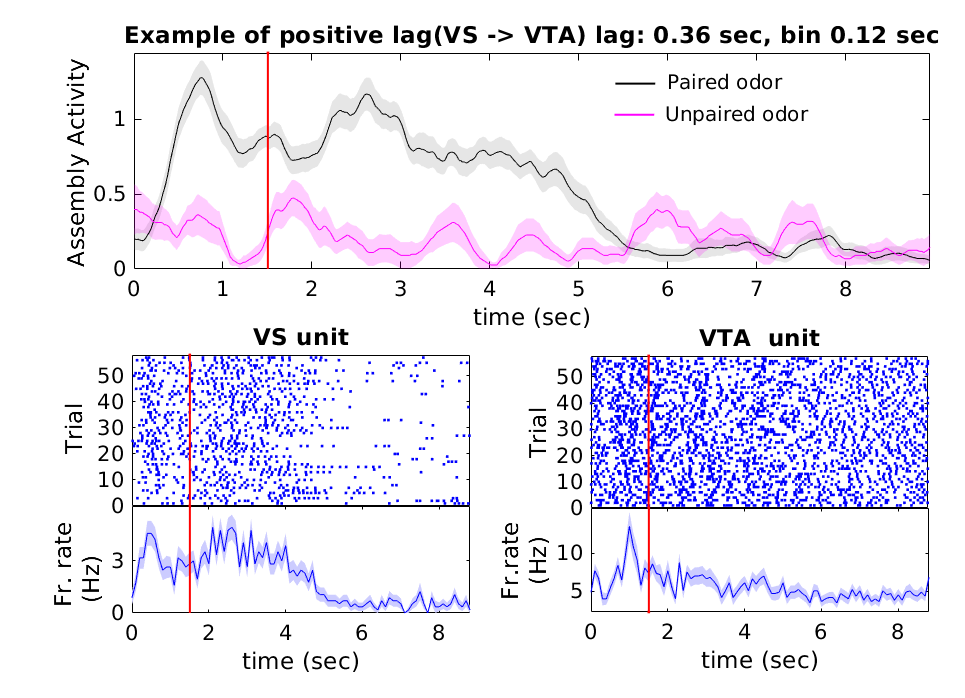
\includegraphics[scale=0.4]{figures/1_21Lastrev1Pru_An4Poster2.png}
    \caption{Directional assembly. On top mean and standard deviation of the assembly's activity for paired (grey) and unpaired odor trials (purple) in the original phase. On bottom raster plot and firing rate (mean and standard deviation) of units in assembly. x-axis origin correspond to the odor onset, while the red line marks the end of the stimulus duration. The examined assembly has a positive lag, that means VS preceding in activity VTA, from neuronal activity we can see in fact the VS unit activate before than the VTA unit.}
    \label{fig:directional_assembly}
\end{figure}
\section{Conclusion}
From the inter-regional time precision distribution (bin size $\Delta$) we deduced that VS-VTA interactions are two time scales interactions. Looking at the assembly activity patterns we observed a dissection between the more precise time scale and the broader time scale inter-regional pairs. 
With the lags between units activation we have distinguished three types of assemblies: synchronous, positive directional and negative directional assemblies. From lag distributions one deduces that precise and broad time scale pairs show directionality in the direction of VS leading VTA.
Directional assemblies are formed by Striatal Projection Neurons and Dopaminergic Neurons.
Does directional assemblies show a different coding features with respect to other assemblies types?
To address this question we first investigate the assemblies task related pattern.
  
 \section{Differences among assemblies types}
 
 %%First difference between original and reversal phase is number of assemblies responding during the post-stimulus interval, this number decrease for all the typologies involved during hit trials (as shown in fig. (\ref{fig:histo_taskrel})), in according to the intuition, in reversal phase in fact, when the animals became more expert, neuronal response tend to be shifted closer to the reward delivery. This effect can be seen in fig. (\ref{fig:NeusInAsse}) where activity and raster plots of two units in a pair are shown. Looking at the raster plots, a shift in correspondence to the phase-switch is evident in both units.
 %\begin{figure}
  %   \centering
  %   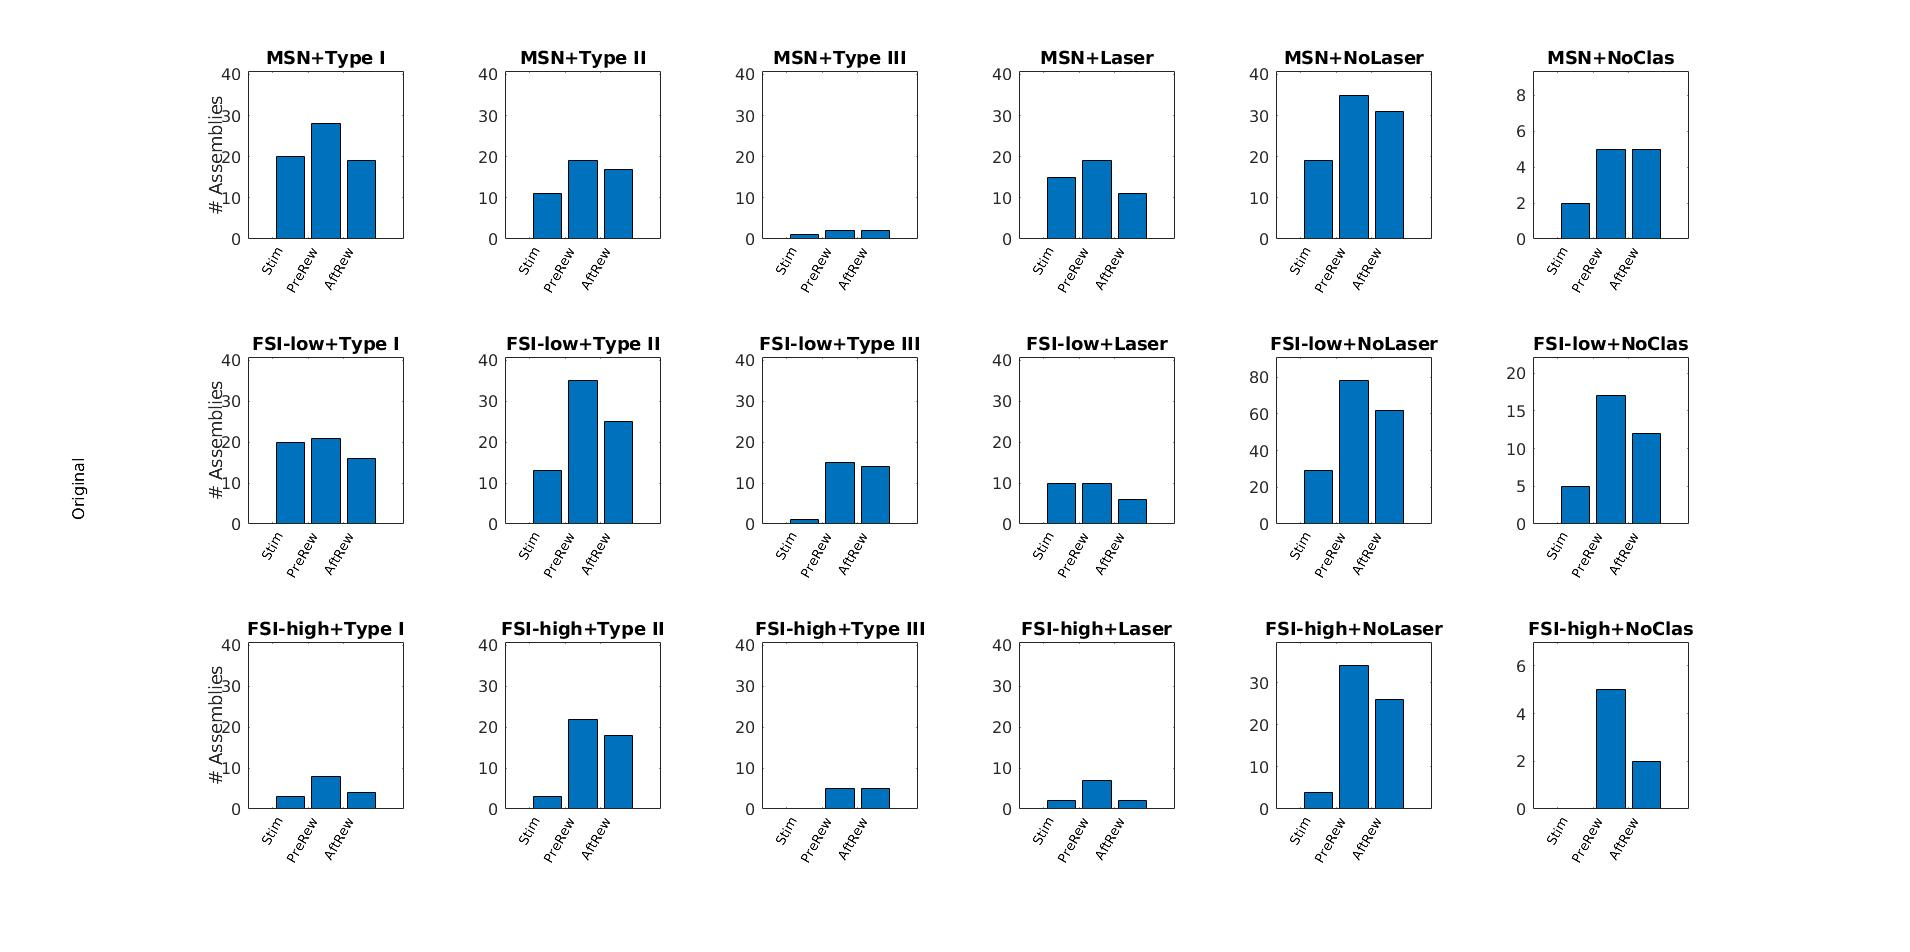
\includegraphics[scale=0.3]{figures/Original_Hit_N.jpg}
    % 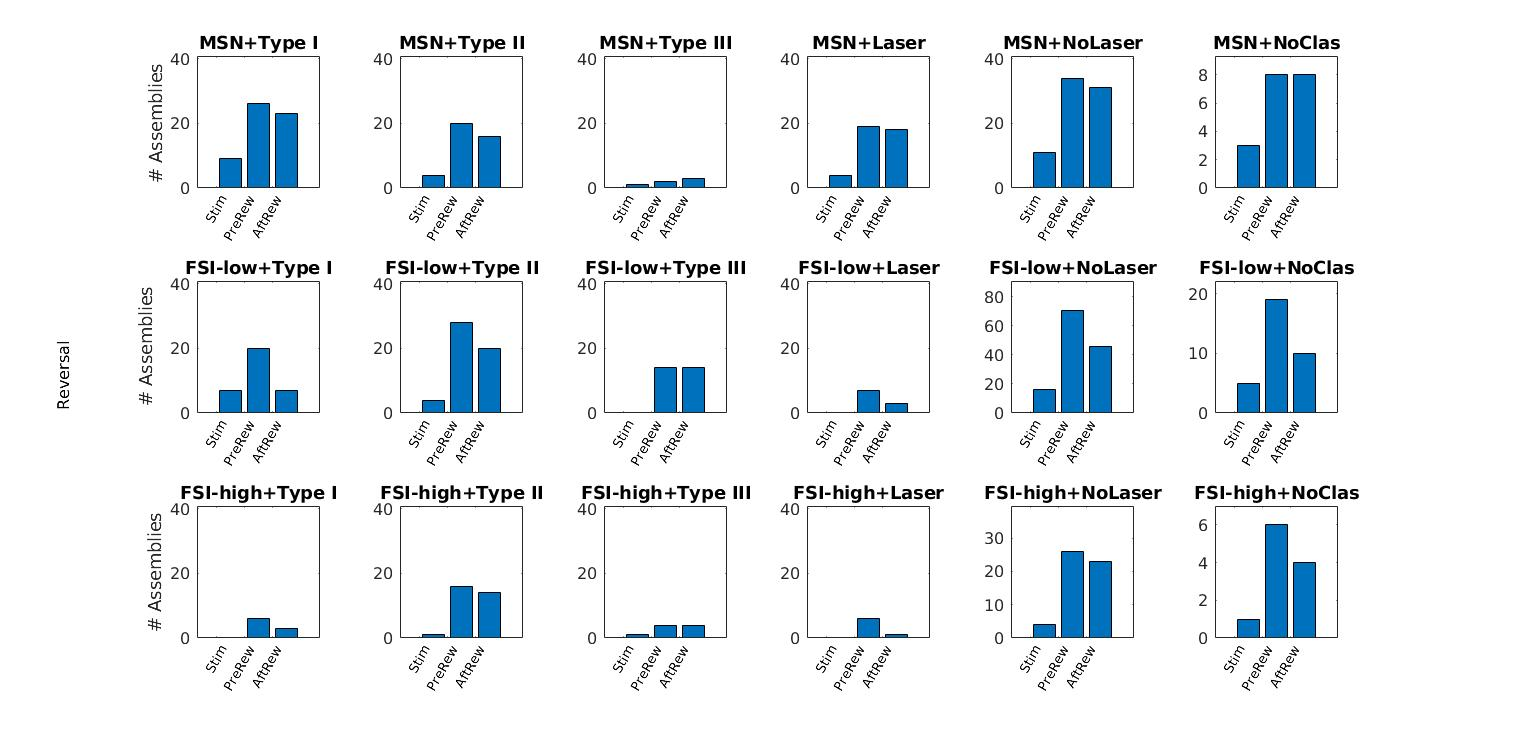
\includegraphics[scale=0.3]{figures/Reversal_Hit_N.jpg}
     %\caption{{\color{red}TO MODIFY!!!! BUT THIS IS THE PLOT}}
     %\label{fig:histo_taskrel}
 %\end{figure}
%\begin{figure}
  %  \centering
   % 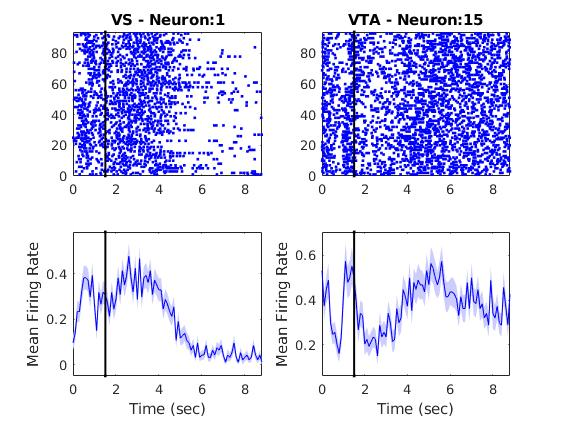
\includegraphics[scale=0.6]{figures/SingleNeus1_15Lastrev1Pru_An_4.jpg}
    %\caption{Shift in time of neuronal activity of two units in assembly. }
    %\label{fig:NeusInAsse}
%\end{figure}

%\section{Discussion}
%\section{Combination of single neuron and assemblies analysis}
%\subsection{Directionality using classification}
%\subsection{Significant task related response for typology}
To better study assemblies activation patterns, first the task relevant moments of the experiment were selected. From the mean task related activity patterns we expected to see differences among assemblies types in two experimental chapters (original and reversal). To better visualize the task related activation patterns via heat plots, hit trials (rewarded odor, mouse went for reward), correct rejection trials (unrewarded odor, mouse sat quiet), false alarm trials (unrewarded odor, mouse went for reward), were kept separated; however this separation among trials types was released in further analysis, without affecting results.
The assemblies were pruned according their significant task related activity, that was tested with Friedman's test and a non parametric version of the repeated measures Anova. We preferred to use non-parametric tests to be free from the assumption of gaussianity of the observations. Results of the two tests were consistent each other. The two relevant events of the task were the odor onset and the reward delivery, then we choose whether the assemblies showed a significant activity in three windows: Stimulus [0s, 0.5s], Pre-Reward [-0.5s, 0s], Reward [0s, 05s], the baseline was chosen in the interval [-1s, -0.5s] from the odor onset. Post-hoc analysis were performed using the Bonferroni's criterion {\color{red}check whether the criterion was Bonferroni of some other}. Almost $80\%$ of the VS-VTA assemblies showed a task related activity significant different from the baseline or from another of the windows considered. Of the significant assemblies $\%$ were composed by MSN-Type I units, $\%$ by FSI low-Type I, $\%$ by FSI high-Type I, $\%$ MSN-Type II, $\%$ by FSI low-Type II, $\%$ by FSI high-Type II, the other possible units combinations constitutes a minority and all toghether were the $\%$ {\color{red} Insert numbers of percentage}.

\section{Conclusion}
